Mobile devices in daily life are equipped with increasingly powerful computing and storage abilities, which enables individual devices to accumulate enormous valuable information. It facilitates a huge number of rising technologies such as edge computing and smart home. Meanwhile, the accumulated data in users' devices can be used to train models for various practical purposes due to the flourishing of machine learning. In traditional machine learning frameworks, data needs to be gathered in a central server in order to execute the learning process. However, most data collected by mobile devices is sensitive. Users usually refuse to send their private data to others, such as a learning center, which impedes the development of distributed learning among common users.

Since the computing ability of mobile devices is powerful enough to run small-scale machine learning tasks, FL~\cite{mcmahan2016communicationefficient}, which is a distributed machine learning framework, was proposed to address the privacy problem in learning tasks. FL is developing rapidly and has an increasing number of applications. For example, Google's keyboard query suggestions~\cite{yang2018applied} project was an effective application of FL. Figure~\ref{fed} illustrates the structure of FL. In each round of FL, parties receive a global model from the server and train their models based on their own data respectively. Afterwards, each party sends the parameters of their models to the server while the server runs a particular aggregation algorithm to compute the global model based on these parameters. In such frameworks, users do not need to send their data to the learning server, and thus the privacy of participants is protected.

Though FL can protect users' privacy, attackers can eavesdrop a party's parameter and then establish the inference attack~\cite{Beyond, Leakage, Nasr19}. Additionally, as the server is provided by an untrusted third party, it can easily obtain all participants' parameters in the aggregation process and conduct the inference attack for the reason that in the conventional FL framework~\cite{Nasr19}, parameters are directly sent to the server, which makes the server gathered all information easily. Therefore, sending parameters to the server directly faces the threat of inference attacks. This kind of attack is quite severe as it can be established by any malicious or semi-honest participant in the FL process. Therefore, how to conduct joint learning without leaking parameters to others comes into focus.

Secure aggregation protocols~\cite{shi2011privacy} enable a group of parties who have private information to compute a function of these private without revealing them. There are many works paid attention to secure aggregation for better solutions~\cite{shi2011privacy,RobustAgg,Bonawitz19,Nike,PrivFL}. For example, Shi \emph{et al}.~\cite{shi2011privacy} utilized homomorphic encryption (HE) methods to achieve secure addition. With the data encrypted, attackers cannot obtain any useful information from leaked messages. Therefore, secure aggregation is suitable for FL, which helps to protect intermediate models' parameters. A trivial solution is to employ HE to implement secure aggregation, however, HE algorithms suffer from low efficiency which is hardly acceptable in FL~\cite{HESurvey}. Differential Privacy (DP) is another feasible method to implement secure aggregation whereas DP based frameworks add noises to the parameters to deceive the attackers and these noises also have an influence on the learning result and reduce accuracy. Moreover, Blockchain-based methods~\cite{DeepChain,Lu2020,On-Device} are also promising, and the generally used consensus algorithms in them can be inspiring. Yet blockchain-based methods are still implement-unfriendly so far.

\begin{figure}[!ht]
    \centering
    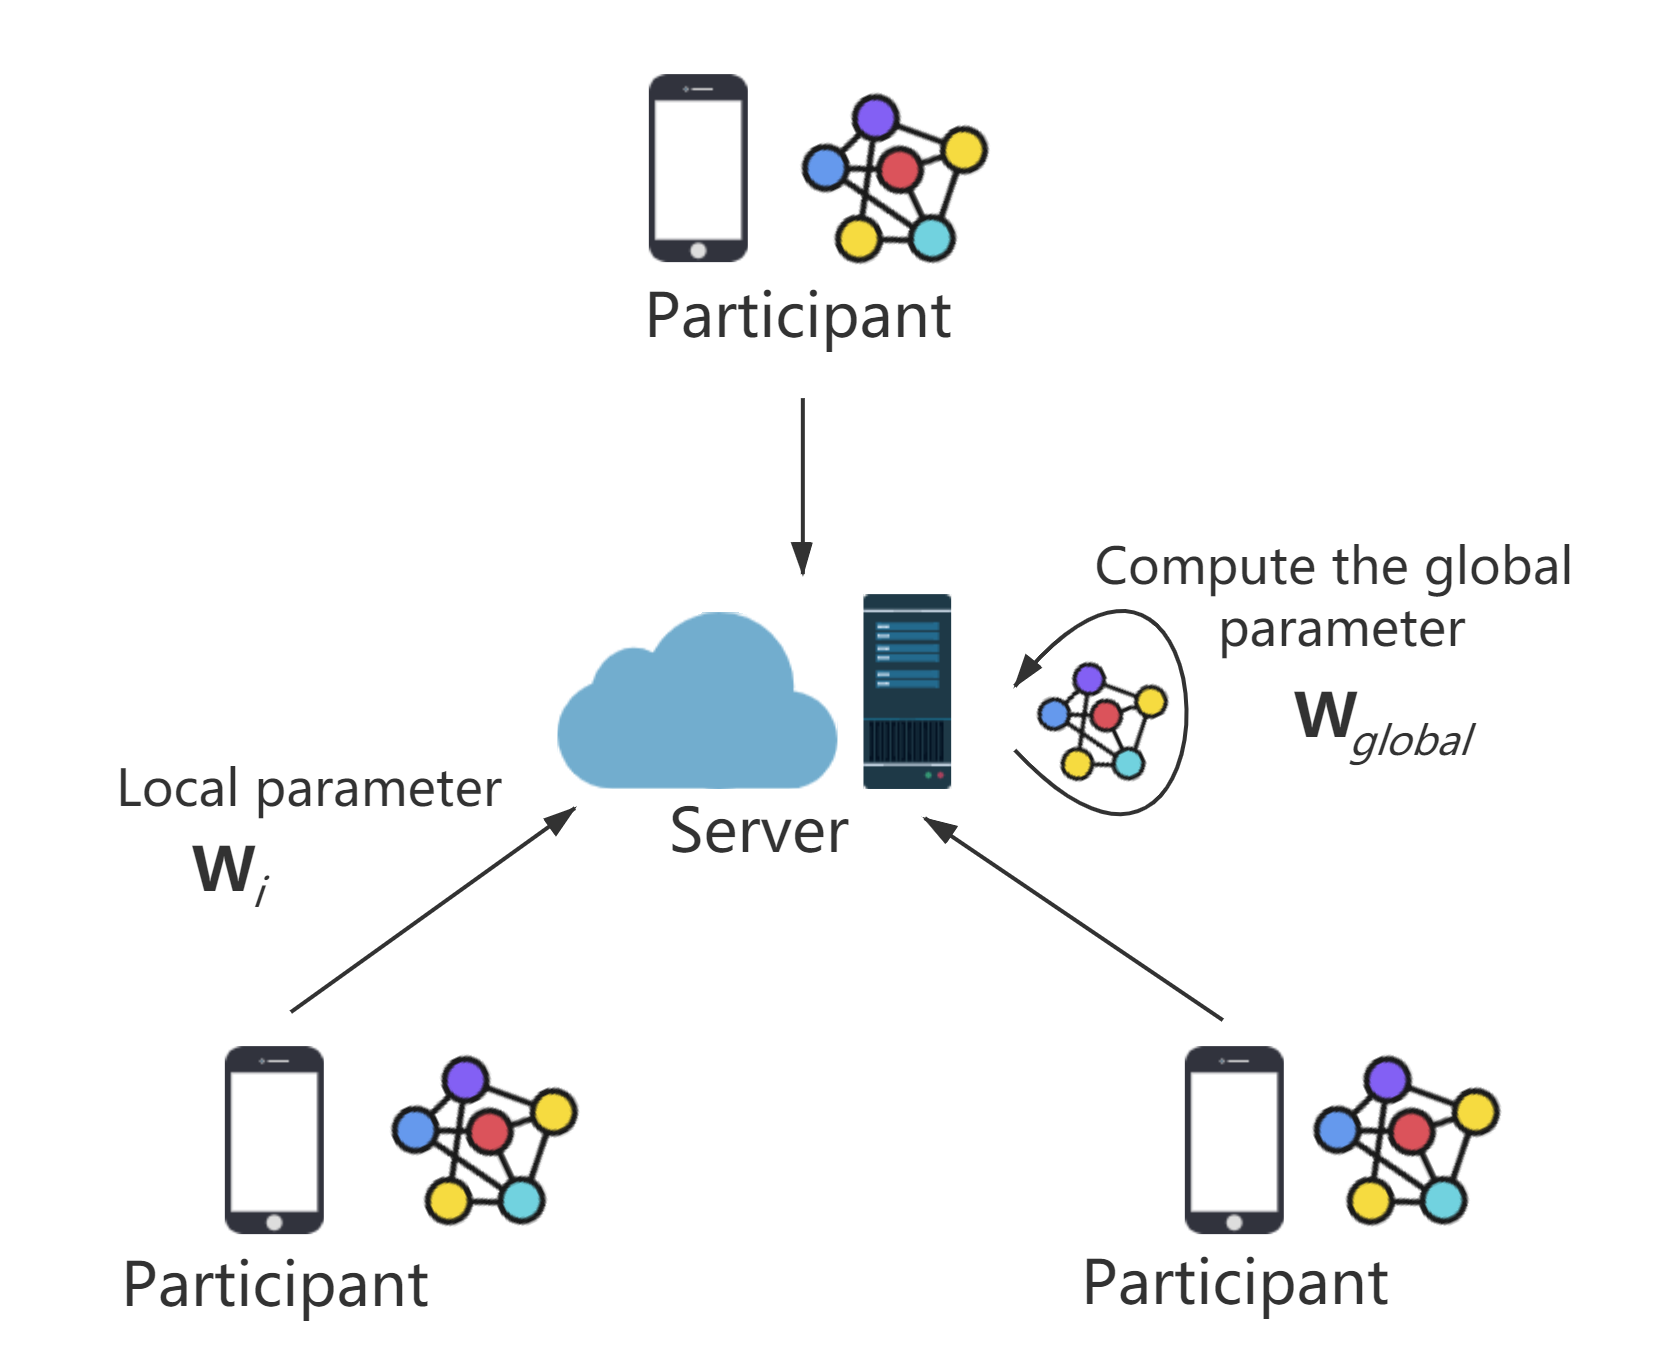
\includegraphics[width=\columnwidth]{img/fed.png}
    \caption{The structure of FL. Participants train local models respectively and send their parameters to the server for aggregation.}
    \label{fed}
\end{figure}

One may think that the multi-party computation (MPC)~\cite{Yao} technique can be leveraged to implement secure aggregation directly. However, most MPC protocols rely on the prerequisite that all participants are able to communicate with each other. In practice, common users of an FL task are unknown to each other, which means one party cannot communicate with another directly. This is a severe obstacle between MPC and FL, therefore, there are some works about realizing P2P communication in FL. For example, Bonawitz \emph{et al}.~\cite{Practical} utilized Diffie-Hellman key exchange to generate pairwise secret masks, however, this method has a dissatisfactory efficiency. The high communication overhead during MPC demands a prompt solution. ~\cite{Two-Phase} also analyzed the MPC process in FL and tried to reduce the overheads by introducing a method based on an aggregation committee, which still has a high price on set-up. In addition, Bonawitz's work also pointed out that the robustness of FL frameworks is also significant because most MPC protocols will fail if there are some participants dropping out, and it usually costs a lot to recover from situations where several nodes are dropping out or crashed. In practice, mobile devices' loss of communication happens frequently, which may cause breakdowns and delays. In summary, employing traditional MPC methods in a system with a large number of users is faced with a problem with efficiency and instability.

\subsection{Motivation} We aim to design a federated learning framework which has these properties:
\begin{enumerate}
    \item It protects users' privacy by employing MPC while solving the problem that participants are unknown to each other.

    \item It has a low communication overhead, avoiding constructing overmuch pairwise connections.

    \item It is secure in semi-honest environments, where all users and the server may eavesdrop information.

    \item It is highly robust, which has the capability to handle emergencies where several participants may lose connection.

    \item It has no negative influence on the quality of the trained model.
\end{enumerate}

\subsection{Our contribution}
\begin{enumerate}
    \item We propose Democratic Federated Learning (DemoFL), a novel FL framework that utilizes MPC to protects users' privacy. DemoFL employs a smart additive secret sharing protocol to realize MPC, which helps to hide intermediate parameters.

    \item DemoFL utilizes hierarchical structure to improve efficiency: our model first selects some leaders, who will construct secure communication with other parties. Afterwards, a party only needs to exchange information with the leaders. The leaders will send the received information to the server, who helps to forward the information to the corresponding destinations. Appointing leaders can reduce the need for communications compared to selecting leaders based on consensus algorithms.

    \item We take advantage of a consensus algorithm to achieve ``democracy'' and high robustness. The consensus algorithm helps to handle unexpected situations where a leader node or a common user is crashed. It selects leaders from all clients democratically and rapidly when such situations happen.

    \item We conducted a series of experiments and verified that DemoFL has satisfactory efficiency and robustness without reducing accuracy.

\end{enumerate}

\subsection{Roadmap} In Section~\ref{sec:back} we introduce the background of knowledge and some definitions. Next, we introduce related work and some platforms of federated learning in Section~\ref{sec:related}. Section~\ref{sec:DemoFL} detailedly illustrates our proposed framework including the attack model. Evaluations for efficiency and security are stated in Section~\ref{sec:eval}, followed with experimental results in Section~\ref{sec:exp}. Finally, we give the conclusion and future expectations in Section~\ref{sec:conc}.